\cleardoublepage
\chapter*{Introduction}
\markboth{Introduction}{Introduction}
\addcontentsline{toc}{chapter}{Introduction}
% Here I bring the reader to general material science background to ML
% applications and their general importance, as well as the the study of
% representations as they are an essential building block

%[R. Tomellini, J. V. Benesch and A. Alming, Commentary: Fostering innovation
%in materials science and engineer].  A material can be more formally described
%by the configurations of atoms and the electron distribution.
%The search for new materials is bound by thermodynamic laws which tell what configurations are stable and can therefore be considered as potential material.
%, i.e. can exist for a limited time frame under a certain set of thermodynamic
%boundary conditions.In the last decades it has been shown that \textit{ab initio} quantum chemistry

In high-throughput materials design, large databases of materials are searched for candidates with desirable characteristics.
So far, searches based on experimental data have been limited in scope due to the vast combinatorial space of materials, the heterogeneous quality of available data, and the difficulty in separating the intrinsic properties of a material from those that are contingent on the processing or synthesis conditions.
In the last decades, it has been shown that ab initio quantum chemistry methods provide approximate stability criteria that are in good agreement with experiments~\cite{jansen2015conceptual} making them a viable tool for the screening of new materials~\cite{ceder1998identification, andersson2006toward, yang2012search, gomez2016design}.
%A viable alternative is to calculate material properties using computer simulations, that make it possible to exploit advances in parallel computing to construct databases with millions of entries, and to obtain results that are internally consistent.
The quantitative accuracy of these predictions, however, is dependent on the quality of the reference electronic structure calculations. 
Higher levels of theory are often necessary to model the electronic structure properties correctly, but they come with an additional computational effort, thereby reducing the breadth of the searches.
Due to the vast number of possible atomic structures to be considered, the efficiency of these methods is crucial.
Data-driven methods have become an efficient extension, reducing expensive quantum chemistry calculations to a bare minimum while reaching close-to-ab initio accuracy over a wide configuration space~\cite{bartok2018machine}, leading to the exploration of previously computationally intractable problems, such as the thermal conductivity of amorphous germanium telluride~\cite{sosso2012thermal}, and moving simulations more into the role as guidance for experiments~\cite{chang_simulations_2023}.
These methods are based on transforming geometrical, physical, and chemical information into a vector representation, referred to as descriptor, to then use it as input of a machine learning mode as shown in the schematic in Figure~\ref{fig:high-throughput-scheme}.
The development of expressive and computationally inexpensive descriptors~\cite{kabylda2023efficient, doi:10.1021/acs.chemrev.0c01111} has led to applications in a wide range of areas~\cite{mansouri2018machine, sosso2018understanding, basdogan2019machine}.
Efficient descriptors are therefore essential for state-of-the-art high-throughput material design applications.
The efficient computation of expressive descriptors is a challenging problem that has seen a wide range of proposals~\cite{behl11jcp, rupp2012fast, bart+13prb, huo2017unified}.
%It has been shown that density-based state-of-the-art descriptors can be seen as different representations of the symmetrized many-body correlation function~\cite{willatt2019atom}.
When used to build an interatomic potential or to predict other atomic-scale properties, representations are used together with different supervised learning schemes, so it is difficult to disentangle the interplay of the descriptor, regression method, and target property that combine to determine the accuracy and computational cost of the different methods~\cite{zuo+20jpcl}.
A deeper understanding of these descriptors is therefore essential, especially considering that the efficiency of accurate potentials is still a limiting factor for the research that can be conducted on materials.

In the first chapter of this thesis, atomistic descriptors based on geometrical information and developed in the last two decades are formalized in a mathematically grounded theory utilizing concepts of representation theory to connect the set of numerical descriptions to functional spaces. %, namely the atomic-centered denstiy correlation function.
In the second chapter, we continue to present a set of measures that can serve for quantitative analysis to guide the choice of the descriptor and model and to provide insight into the inherent nature of the descriptors.
Insights are presented on how changes in the smearing, cutoff, radial scaling, body-order or switch of the metric space to the Wasserstein metric affects the information content of the feature space induced by the metric.
%with relationship to features induced the Euclidean distance.
%, that can represent distances between distant distrubtions more faithfully, 
In Chapter~\ref{sec:basisopt} we present how symmetries can be embedded into data-driven optimization methods based on the covariance or correlation matrix to improve the radial basis functions.
The information capacity is evaluated with the metrics developed in Chapter~\ref{sec:infocap} and benchmarks on the regression performance for a single species and a multi-species dataset are shown.
The last chapter focuses on the implementation of a machine learning interatomic potential (MLIP) and showcases its application to study finite-size effects in paraelectric-ferroelectric phase transitions in barium titanate.
The specifications of the spline used for the basis optimization presented in Chapter~\ref{sec:mlip} are written out, and the effect of the grid on performance and accuracy is briefly discussed.
Finally, drawbacks in extensibility and deployment of the developed MLIP software are outlined, and future directions for a modular machine learning software ecosystem for atomistic simulations are presented.

%exploit the, for the widely-applied GAP model
%covering on one hand the efficient implementation of descriptors and data-driven models, and on the other hand their deployment into molecular dynamics software.
 

\begin{figure}
    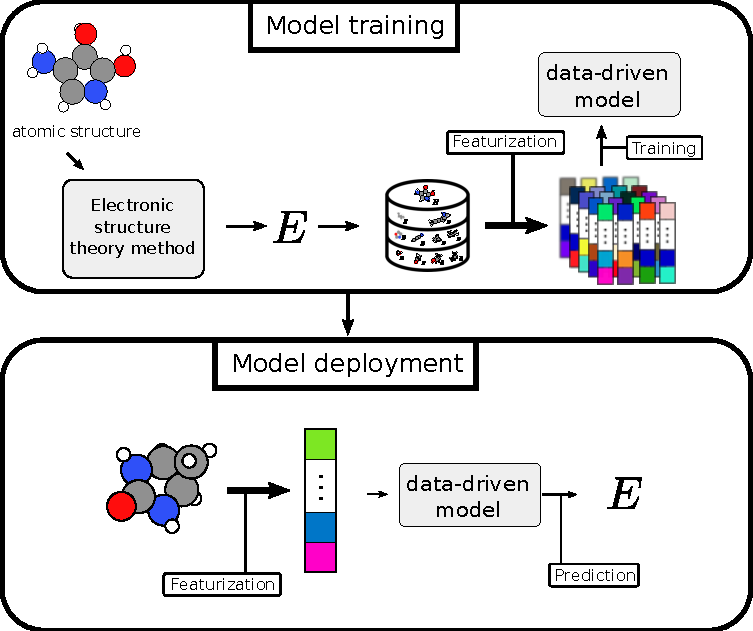
\includegraphics[width=\textwidth]{fig/highthroughput-scheme.pdf}
    \caption{A schematic showing the idea of high-throughput calculations with a data-driven model that serves as surrogate model to bypass the expensive electronic structure theory calculations after training the model.}
    \label{fig:high-throughput-scheme}
\end{figure}
%The key conceptual/domain part behind the methods determining their quality is
%the choice of description of the configuration called descriptor and the way
%to express similarity between these descriptions.

%0.5 page Statement of the problem and specific problem:
%considering that blackbox machinaries as neural networks make it hard to specify what information contributed to their success making the improvement of models similar to try to hit a bin with a rock that lies in completely in the shadows.
%While neural networks have been successful in pushing the limits in inference accuray, due to their highly parametric nature they cannot compete with splining techniques.
%We have to take one step back and ask us do we really need this?



%The continuation of this development is the objective of this thesis.  The
%general goal of the thesis is the improvement of state of the art descriptors
%in terms of their encoded information and their concrete implementations.
%Since machine learning models are based on comparing features with the help of
%a similarity measurement, there is a strong connection between the similarity
%of two atomic configurations in form of their descriptor, and the Euclidean
%distance between their symmetrized many-body correlation function.
%The general goal of the thesis is the improvement of state of the art
%descriptors in terms of their encoded information and their concrete
%implementations.
%While the Euclidean distance can represent distances between close
%distributions accurately, more distant ones are not faithfully represented.
%On the other hand descriptors relying on sorting geometric
%information\cite{rupp2012fast, gallet2013structural} are similarly connected to
%the Wasserstein distance\cite{rowland2019orthogonal}.  The effect of the
%distance among atomic environments on the descriptor and subsequently on the
%regression of physical properties has not been extensively analyzed yet and is
%part of the objective of this thesis.  Such an analysis requires the
%development of measures for the comparison of feature spaces and efficient
%adaptations of the Wasserstein distance to a wider range of descriptors.

%Furthermore, recently generative models have been introduced for the generation
%of stable atomic configurations\cite{Sanchez-Lengeling360, gebauer2019symmetry,
%noe2019boltzmann, hoffmann2019data}.  The usage of descriptors in generative
%models requires a mapping of the descriptor back to the atomic configuration.
%Heretofore efficient inversion schemes have been introduced only for the
%3-dimensional atomic density function\cite{Sanchez-Lengeling360} and for
%distributions over distances between atoms\cite{gebauer2019symmetry}.  The
%development of an efficient inversion for state of the art descriptors which
%capture translational and rotational invariant many-body order information is
%an open problem which will be addressed with this thesis.
